Of the many advantages conferred by sleep, this thesis will primarily examine sleep’s impact on memory. To provide context, an overview of memory systems and processes will be provided. The subsequent discussion will delve into the crucial role that sleep plays in memory, citing prominent theories that support this claim.

\subsection{Memory systems}
The notion that memory is not a single entity has been acknowledged for a long time. However, the first empirical evidence to support this idea was presented by Brenda Milner in 1957 through her study of the patient H.M., who underwent a bilateral resection of the medial temporal lobe to treat intractable epilepsy. Surprisingly, after the surgery, he was still able to learn new tasks, such as hand-eye coordination, even though he had no recollection of previous learning experiences \parencite{squire_conscious_2015}. This finding indicated that memory is not confined to a single structure but is instead composed of multiple systems that rely on different neuroanatomical structures. A comprehensive overview of the various types of memory has been reported by Henke \parencite{henke_model_2010} and it is depicted in Figure \ref{fig:LTM}. 

\FloatBarrier
\begin{figure}
    \centering    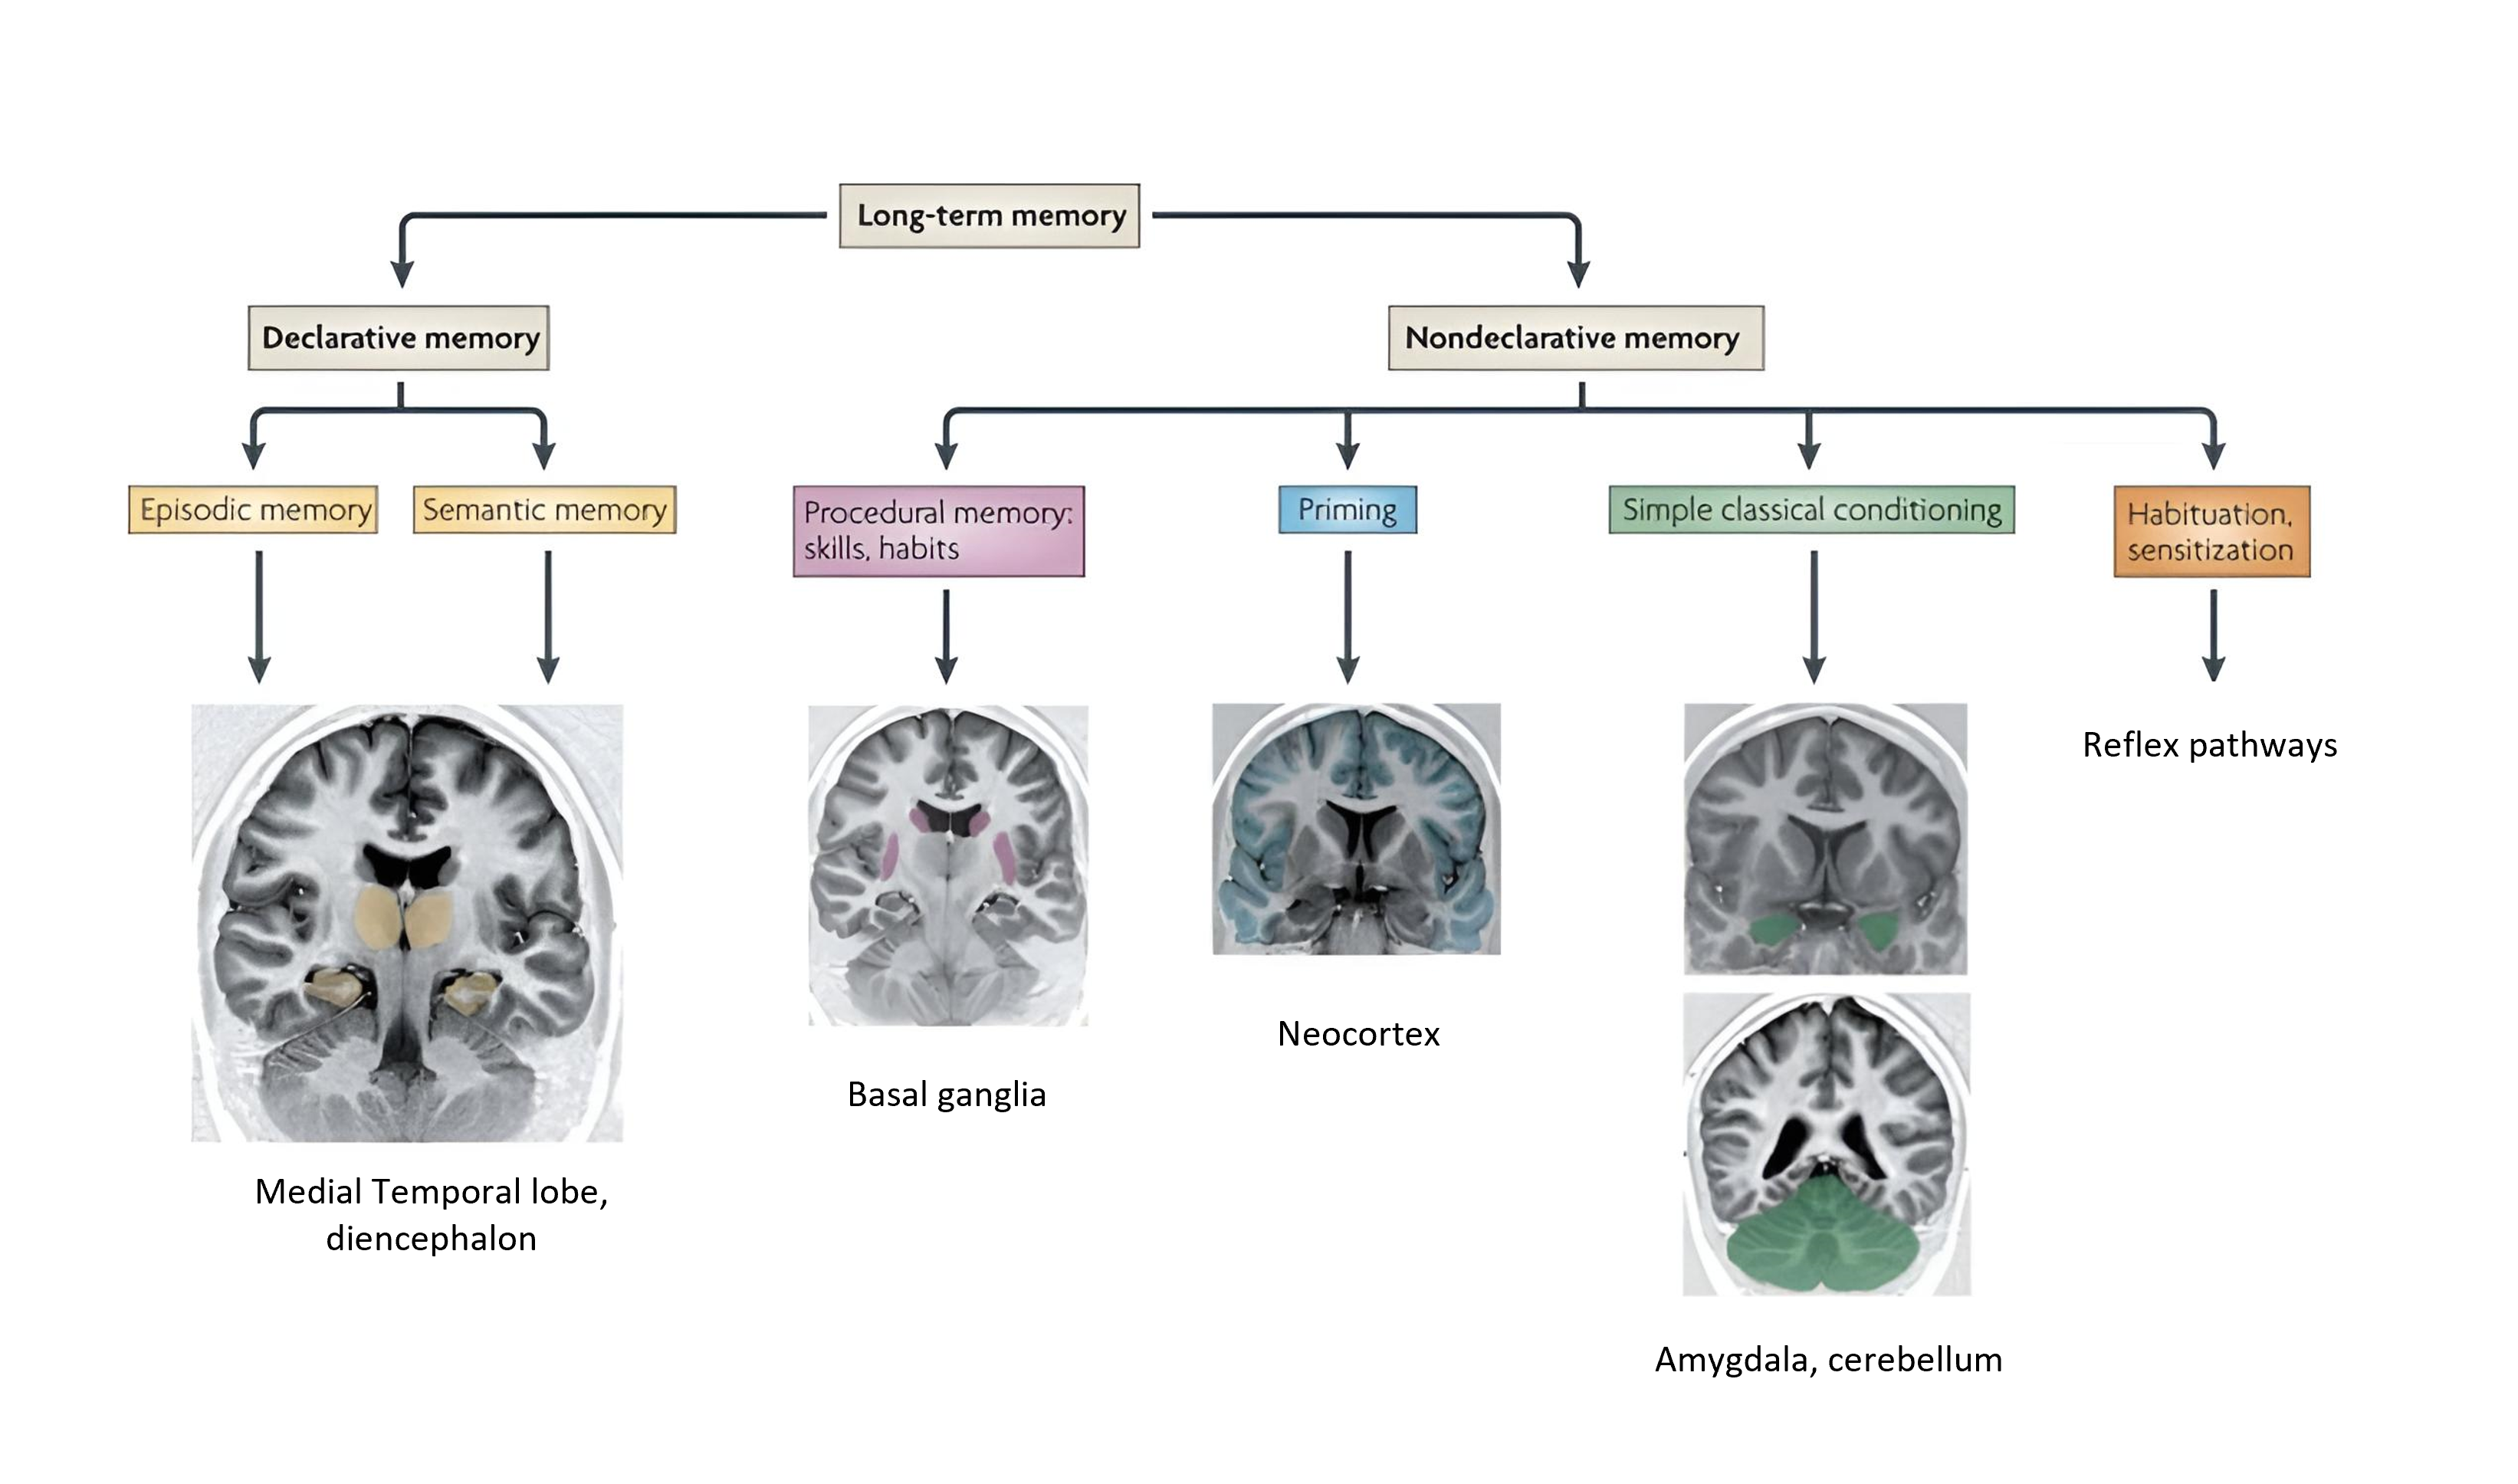
\includegraphics[width=0.9\linewidth]{1_Introduction//IntroImages/LTM.jpg}
    \caption[\textit{Organisation of long-term memory systems and associated brain structures}]{\textit{Organisation of long-term memory systems and associated brain structures.} Modified from \cite{henke_model_2010}. \vspace{1cm}}
    \label{fig:LTM}
\end{figure}

\FloatBarrier

The above figure illustrates the categorization of long-term memory into two primary types: declarative (explicit) and nondeclarative (implicit) memory \parencite{henke_model_2010,squire_conscious_2015,squire_structure_1996}. Declarative memory refers to the conscious recollection of information, and it can be further subdivided into memories for facts (semantic memory) and memories for events (episodic memory). Semantic memory refers to memories of information stored in the absence of contextual knowledge, whereas episodic memory is embedded in a specific spatiotemporal context. Non-declarative memories are instead linked to unconscious learning and retrieval capacities, and they can be classified into several subtypes. \\
The first subtype, procedural memories, refers to the learning of skills, such as riding a bike or playing an instrument; the second, priming, involves performance enhancement due to prior exposure to related information; the third, conditioning, involves the association of two unrelated stimuli to learn a new response; and finally, non-associative learning refers to the attenuation or augmentation of a response towards a repeated presentation of a stimulus \parencite{henke_model_2010,rasch_about_2013,squire_conscious_2015,squire_structure_1996}. The integrity of the medial temporal lobe system, which includes the hippocampus and entorhinal, perirhinal, and parahippocampal cortices, is thought to be essential for declarative memories. In contrast, nondeclarative memories are generally considered to be hippocampus-independent \parencite{squire_conscious_2015,squire_structure_1996}.
\FloatBarrier



\subsection{Memory processes}\label{Intro:sec:Memory processes}
Memory is formed over time through three distinct processes: encoding, consolidation, and retrieval. 
Encoding comprises the formation of new memory traces following the perception of a stimulus. These newly encoded traces are initially labile and susceptible to chance and forgetting, but they become increasingly robust and resistant to interference through consolidation. During this process, the new memory traces are integrated into pre-existing long-term memory networks \parencite{rasch_about_2013}.

\textit{Consolidation} involves two steps: synaptic and system consolidation. The initial step is accomplished at a synaptic level within minutes or hours after learning and leads to enduring changes in synaptic connections \parencite{kandel_molecular_2001}. Synaptic consolidation is then supplemented by system consolidation which redistributes synaptic connectivity across different brain areas \parencite{frankland_organization_2005}. These changes enable the newly encoded information to become part of long-term memory, providing a basis for later retrieval \parencite{rasch_about_2013}. However, two significant challenges arise: how newly learned material becomes permanently accessible without overwriting old memories, and how the brain determines what information to store or forget. 

The \textbf{standard two-stage model of memories} \parencite{marr_simple_1971} offered a solution to the first issue, and nowadays, it constitutes the most influential model of human memory. The model suggests that effective learning requires two complementary systems: the hippocampus and the neocortex. During wakefulness, the hippocampus acts as a fast-learning storage where new memory traces are temporarily stored. These memories are gradually transferred into the neocortex, a long-term slow-learning storage system. The model further proposes that the transfer process (from the short-term store to the long-term one) occurs slowly via repeated and spontaneous reactivation of hippocampal-cortical networks. Over time, network reactivation increases the stability and strength of cortico-cortical connections, allowing integration of the traces into pre-existing neocortical knowledge networks. Ultimately, this results in memories becoming hippocampal-independent \parencite{frankland_organization_2005,marr_simple_1971,squire_retrograde_1995}. These complementary memory systems allow the storage of new memories without interfering with existing ones.

With respect to the second challenge - how the brain determines what information to store or forget - it seems sensible that information in some way relevant for adapting to the environment or important for upcoming challenges will be preferred. In this context, emotions have been shown to play a significant role in labelling which information will be stored in memory and which will be forgotten \parencite{dolan_emotion_2002,williams_power_2022}. Numerous studies have demonstrated that emotional stimuli are better remembered than their neutral counterparts, largely due to the modulatory role played by the amygdala in the process of hippocampal-dependent memory formation \parencite{anderson_neural_2003,mcgaugh_memory_2000,mcgaugh_role_2002,vuilleumier_effects_2001,whalen_masked_1998}. Indeed, during the initial encoding phase, the amygdala rapidly responds to emotional stimuli, often before conscious awareness, thereby enhancing attention to prioritise the processing of these stimuli. In later stages of memory formation, it modulates the effects of stress hormones in the consolidation of hippocampal-dependent memories \parencite{diano_amygdala_2017,phelps_human_2004}. As a result, emotionally charged events are more readily remembered. 

The hippocampo-cortical information transfer of memories is a continuous process that occurs not only during wakefulness but also during offline periods including sleep. Sleep, indeed, is an ideal time window for these processes to occur as it protects memories from interference by preventing encoding of new information \parencite{ellenbogen_role_2006,rasch_about_2013}.
\FloatBarrier



\subsection{Models of sleep and memory}\label{Intro:sec:Models of sleep and memory}
Although as early as 1885 Ebbinghaus published a seminal study demonstrating the effect of time on forgetting (i.e. forgetting is reduced when followed by a period of sleep), the interest in studying the relationship between sleep and memory was reignited only in the late 1980s with a variety of studies demonstrating the beneficial effects of NREM and REM sleep on memory consolidation \parencite[see][for a review]{rasch_about_2013}. A differential role of these two sleep stages in the consolidation of different types of memory was theorised by the \textbf{Dual Process Hypothesis} \parencite{gais_declarative_2004,rasch_about_2013,smith_sleep_2001}. This account assumes that hippocampus-dependent declarative memories are linked to NREM sleep, while REM sleep benefits the consolidation of nondeclarative memories, such as procedural and emotional. The Dual process hypothesis is supported by human studies that employed the “night–half paradigm”, in which participants’ memory performance is compared across retention intervals including the early half (rich in NREM sleep) and the late half of the night (rich in REM sleep). However, this methodology overlooks the fact that neither the early nor the late half of the night contains one stage of sleep. Furthermore, subsequent experiments have not consistently demonstrated this distinction \parencite[e.g.,][]{fogel_dissociable_2007,huber_arm_2006,rauchs_consolidation_2004}, and theoretical accounts have proposed that the cyclic succession of NREM and REM sleep may constitute the key to successful overnight memory consolidation. 

The \textbf{Sequential hypothesis} \parencite{ambrosini_learning_2001,giuditta_sequential_1995} stresses this concept and assumes that during SWS, non-adaptive or irrelevant memory traces are downscaled (or eliminated), while useful memories are strengthened. Subsequently, during REM sleep, these adaptive memories are integrated with pre-existing memories. Supporting evidence for the Sequential hypothesis has been originally obtained from studies conducted with animals \parencite[e.g.,][]{ambrosini_sequential_1992,ambrosini_sequential_1995} and then confirmed in humans \parencite[e.g.,][]{ficca_morning_2000,mednick_sleep-dependent_2003,stickgold_visual_2000}. For example, Ficca and colleagues investigated the impact of sleep cycle disorganisation on the recall of verbal material in young adults and demonstrated that morning recall was significantly affected by sleep cycle disorganisation \parencite{ficca_morning_2000}.

The \textbf{Active System Consolidation Hypothesis} \parencite[ASC,][Figure \ref{fig:ASC}]{diekelmann_memory_2010,rasch_about_2013} represents the most prominent model in the field. It originates from the Standard two-stage model of memories (see section \ref{Intro:sec:Memory processes}) and argues that sleep is not merely a passive state but is actively involved in memory consolidation. Furthermore, central to this model is the concept that newly encoded memory representations are repeatedly reactivated during sleep, a vital process for consolidation. During encoding, labile memory traces are stored temporarily in the hippocampus. Subsequently, during SWS, these traces undergo repeated reactivation, facilitating their gradual transfer to the cortex for long-term storage (Figure \ref{fig:ASC}A). The involvement of SWS in memory processing is well-documented \parencite{diekelmann_memory_2010, walker_role_2009, rasch_about_2013}, highlighting its importance in this model.
A critical aspect of the transfer of memory traces involves the precise temporal synchronization of three key oscillations during SWS: neocortical slow oscillations, thalamo-cortical spindles, and hippocampal sharp wave ripples (Figure \ref{fig:ASC}B). The SOs up-states trigger memory reactivations in tandem with hippocampal ripples. Ripples have been shown to occur in the troughs of spindles, which are in turn coupled with the SOs up-states. This intricate coupling is essential for the efficient transfer of reactivated memory traces, thereby facilitating their integration into the neocortex \parencite{rasch_about_2013}. 

\FloatBarrier
\begin{figure}
    \centering
    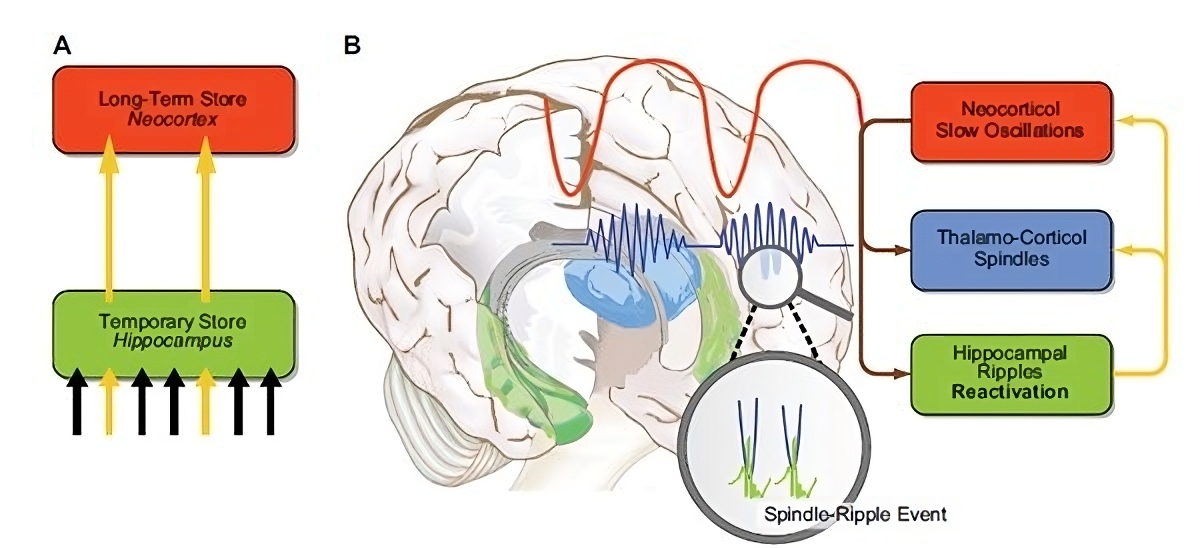
\includegraphics[width=0.9\linewidth]{1_Introduction//IntroImages/Picture4-K7_mBWyR6-transformed.jpeg}
    \caption[\textit{The Active System Consolidation Hypothesis}]{\textit{The Active System Consolidation Hypothesis.} \textbf{(A)} Newly acquired memories are encoded into a temporary store, the hippocampus, and transferred to the long-term neocortical store during SWS. \textbf{(B)} The cortico-hippocampal dialogue is orchestrated by neocortical slow oscillations (red), thalamo-cortical spindles (blue), and hippocampal sharp-wave ripples (green). Source: \cite{rasch_about_2013}. \vspace{1cm}}
    \label{fig:ASC}
\end{figure}
\FloatBarrier

The hypothesis further suggests that the temporal synchronization of SWS-related oscillations not only supports memory reactivation but also leads to a qualitative reorganization of memories, involving their redistribution and transformation. Additionally, REM sleep contributes to the stabilization of these transferred memories through synaptic consolidation. Empirical evidence from various studies bolsters this hypothesis. For example, research in rodents using paradigms like fear conditioning or object recognition tasks has demonstrated the necessity of this coupling for effective consolidation \parencite{maingret_hippocampo-cortical_2016, latchoumane_thalamic_2017}. Similarly, human intracranial EEG recordings in epilepsy patients have corroborated these findings \parencite{helfrich_bidirectional_2019, jiang_posterior_2019}. Finally, the coupling between SOs and spindles was shown to correlate with performance improvements on several memory tasks \parencite[for instance][]{schreiner_endogenous_2021, muehlroth_precise_2019, hahn_slow_2020}.

An alternative hypothesis for the mechanisms underlying memory consolidation during sleep has been offered by the \textbf{Synaptic Homeostasis Hypothesis} \parencite[SHY,][Figure \ref{fig:SHY}]{tononi_sleep_2003,tononi_sleep_2006}. It postulates that wakefulness is accompanied by a net increase in synaptic strength that progressively saturates learning abilities. Sleep, as an antidote, promotes synaptic downscaling, renormalizing the net synaptic strength and restoring the brain’s ability for future encoding (synaptic homeostasis), while maintaining certain memory traces. Further, this renormalization mechanism is proposed to occur during SWA, a hallmark of SWS. This hypothesis has been corroborated by sleep deprivation studies that demonstrated that memory performance is worse after waking than sleep \parencite{ashton_sleep_2020, gais_sleep_2006, yang_repeated_2012} and by studies that highlighted that the amount of SWA predicts memory performance after sleep \parencite{huber_arm_2006, ferrarelli_increase_2019}.
Crucially, SHY suggests that memories tagged as important are weakened less - or relatively strengthened - overnight than irrelevant memories, thus promoting the consolidation and integration of memories \parencite{tononi_sleep_2003,tononi_sleep_2006,tononi_sleep_2014, wilhelm_sleep_2014}.

\FloatBarrier
\begin{figure}
    \centering
    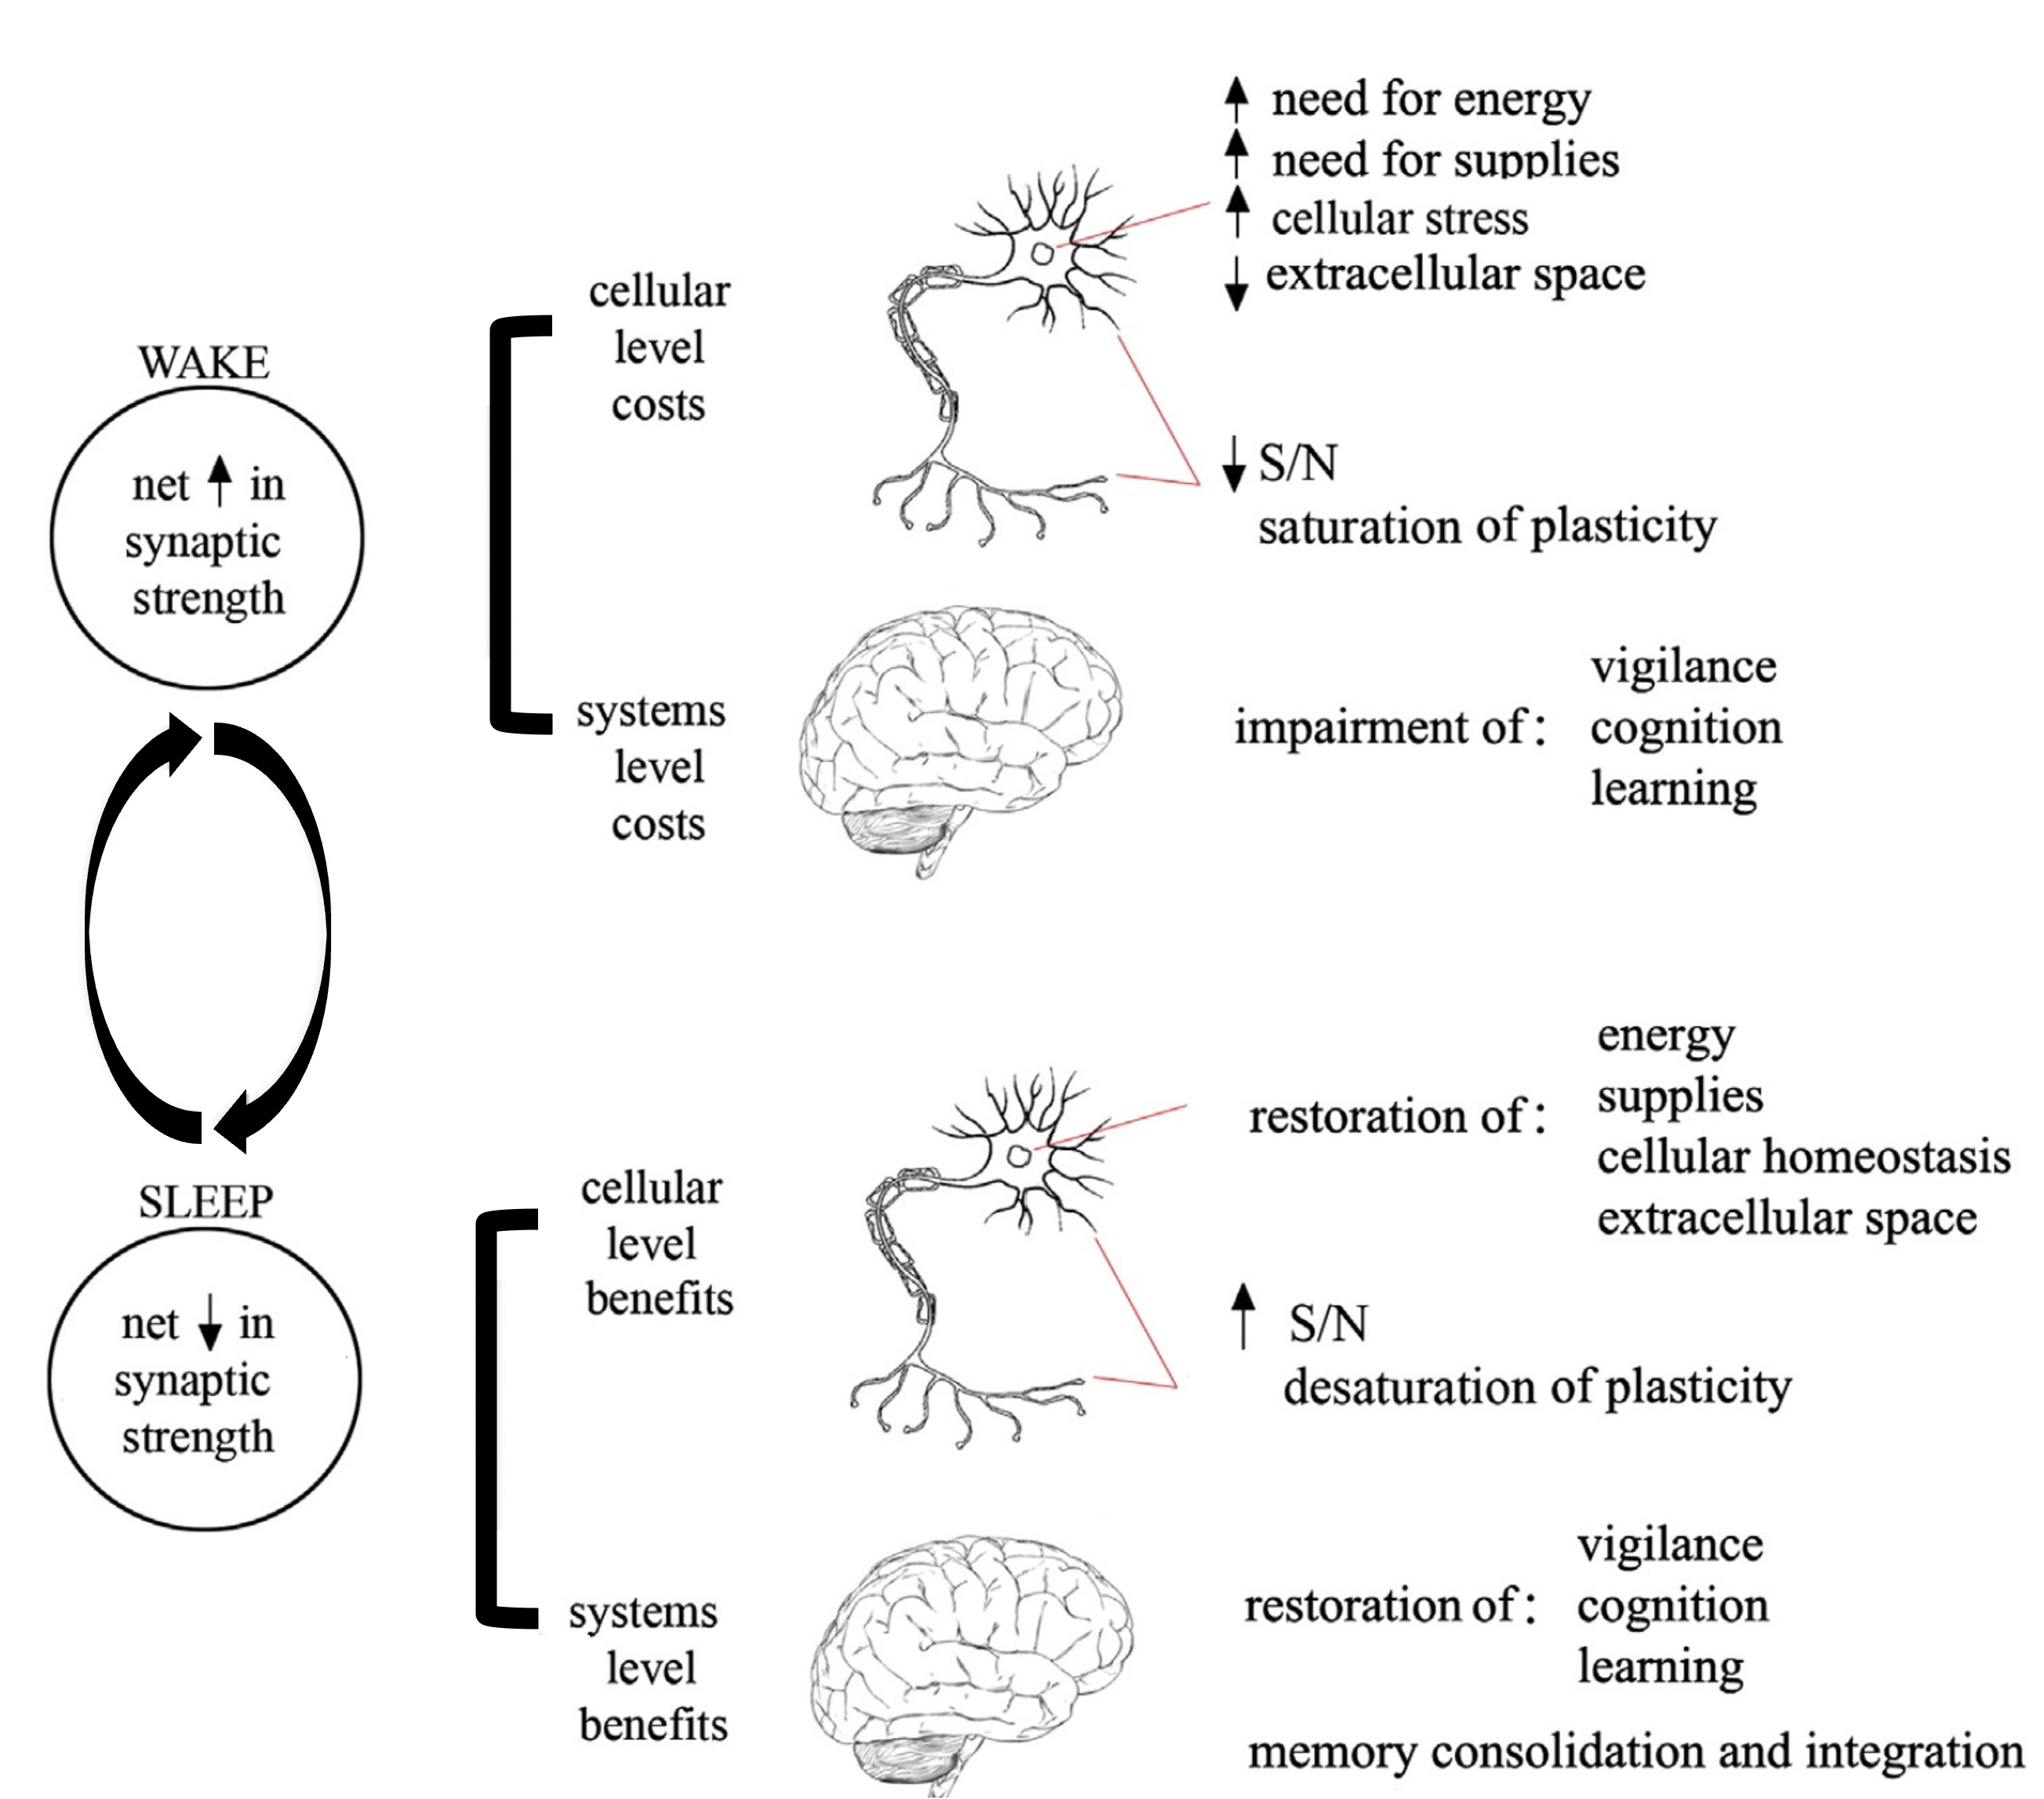
\includegraphics[width=0.8\linewidth]{1_Introduction//IntroImages/Picture5.jpg}
    \caption[\textit{Synaptic Homeostasis Hypothesis}]{\textit{Synaptic Homeostasis Hypothesis.} Modified from \cite{tononi_sleep_2014}. \vspace{0.8cm}}
    \label{fig:SHY}
\end{figure}
\FloatBarrier

There is evidence of a more rapid transfer of information from the hippocampus to the neocortex if the new set of information to be acquired is compatible (overlaps) with an existing framework of organised knowledge, called \textit{schema} \parencite{tse_schemas_2007,van_kesteren_persistent_2010,van_kesteren_retrieval_2010}. The \textbf{Information overlap to abstract} (iOtA) model developed by Lewis and Durrant explains the underlying mechanisms of this facilitation effect and the role sleep plays in it \parencite{lewis_overlapping_2011}. The model states that during SWS, the replay of overlapping memories is strengthened through Hebbian plasticity, representing the core mechanism for schema formation. Synaptic interconnections between neurons that code for shared elements are strengthened and survive SWS downscaling \parencite{abbott_synaptic_2000,lewis_overlapping_2011, tononi_sleep_2003,tononi_sleep_2006}. Thereby, only newly learned information that overlaps with an existing schema and is reactivated on multiple occasions will be potentiated and incorporated into the schema. The replay of overlapping memories in SWS leads to the extraction of commonalities or ‘gist’ (the core of a memory), promoting both a quantitative and a qualitative reorganisation of memory representations \parencite{durrant_sleep-dependent_2011,ellenbogen_human_2007,lewis_overlapping_2011}. The iOtA model is the foundation of the \textbf{Broader Form of the iOtA Model} \parencite[BiOtA]{lewis_how_2018}, which integrates REM sleep into the framework. The BiOtA model emphasizes the significance of the cyclic structure of a night’s sleep, in which NREM and REM alternate. During NREM sleep, the replay of thematically related memories is enhanced, while during REM sleep, the connections between seemingly disparate concepts are recognised, resulting in the formation of new connections between concepts \parencite[Figure \ref{fig:biota};][]{lewis_how_2018}. The interleaving of these two stages could explain the role of sleep in creativity and problem-solving. 
\vspace{1cm}
\begin{figure}[H]
    \centering
    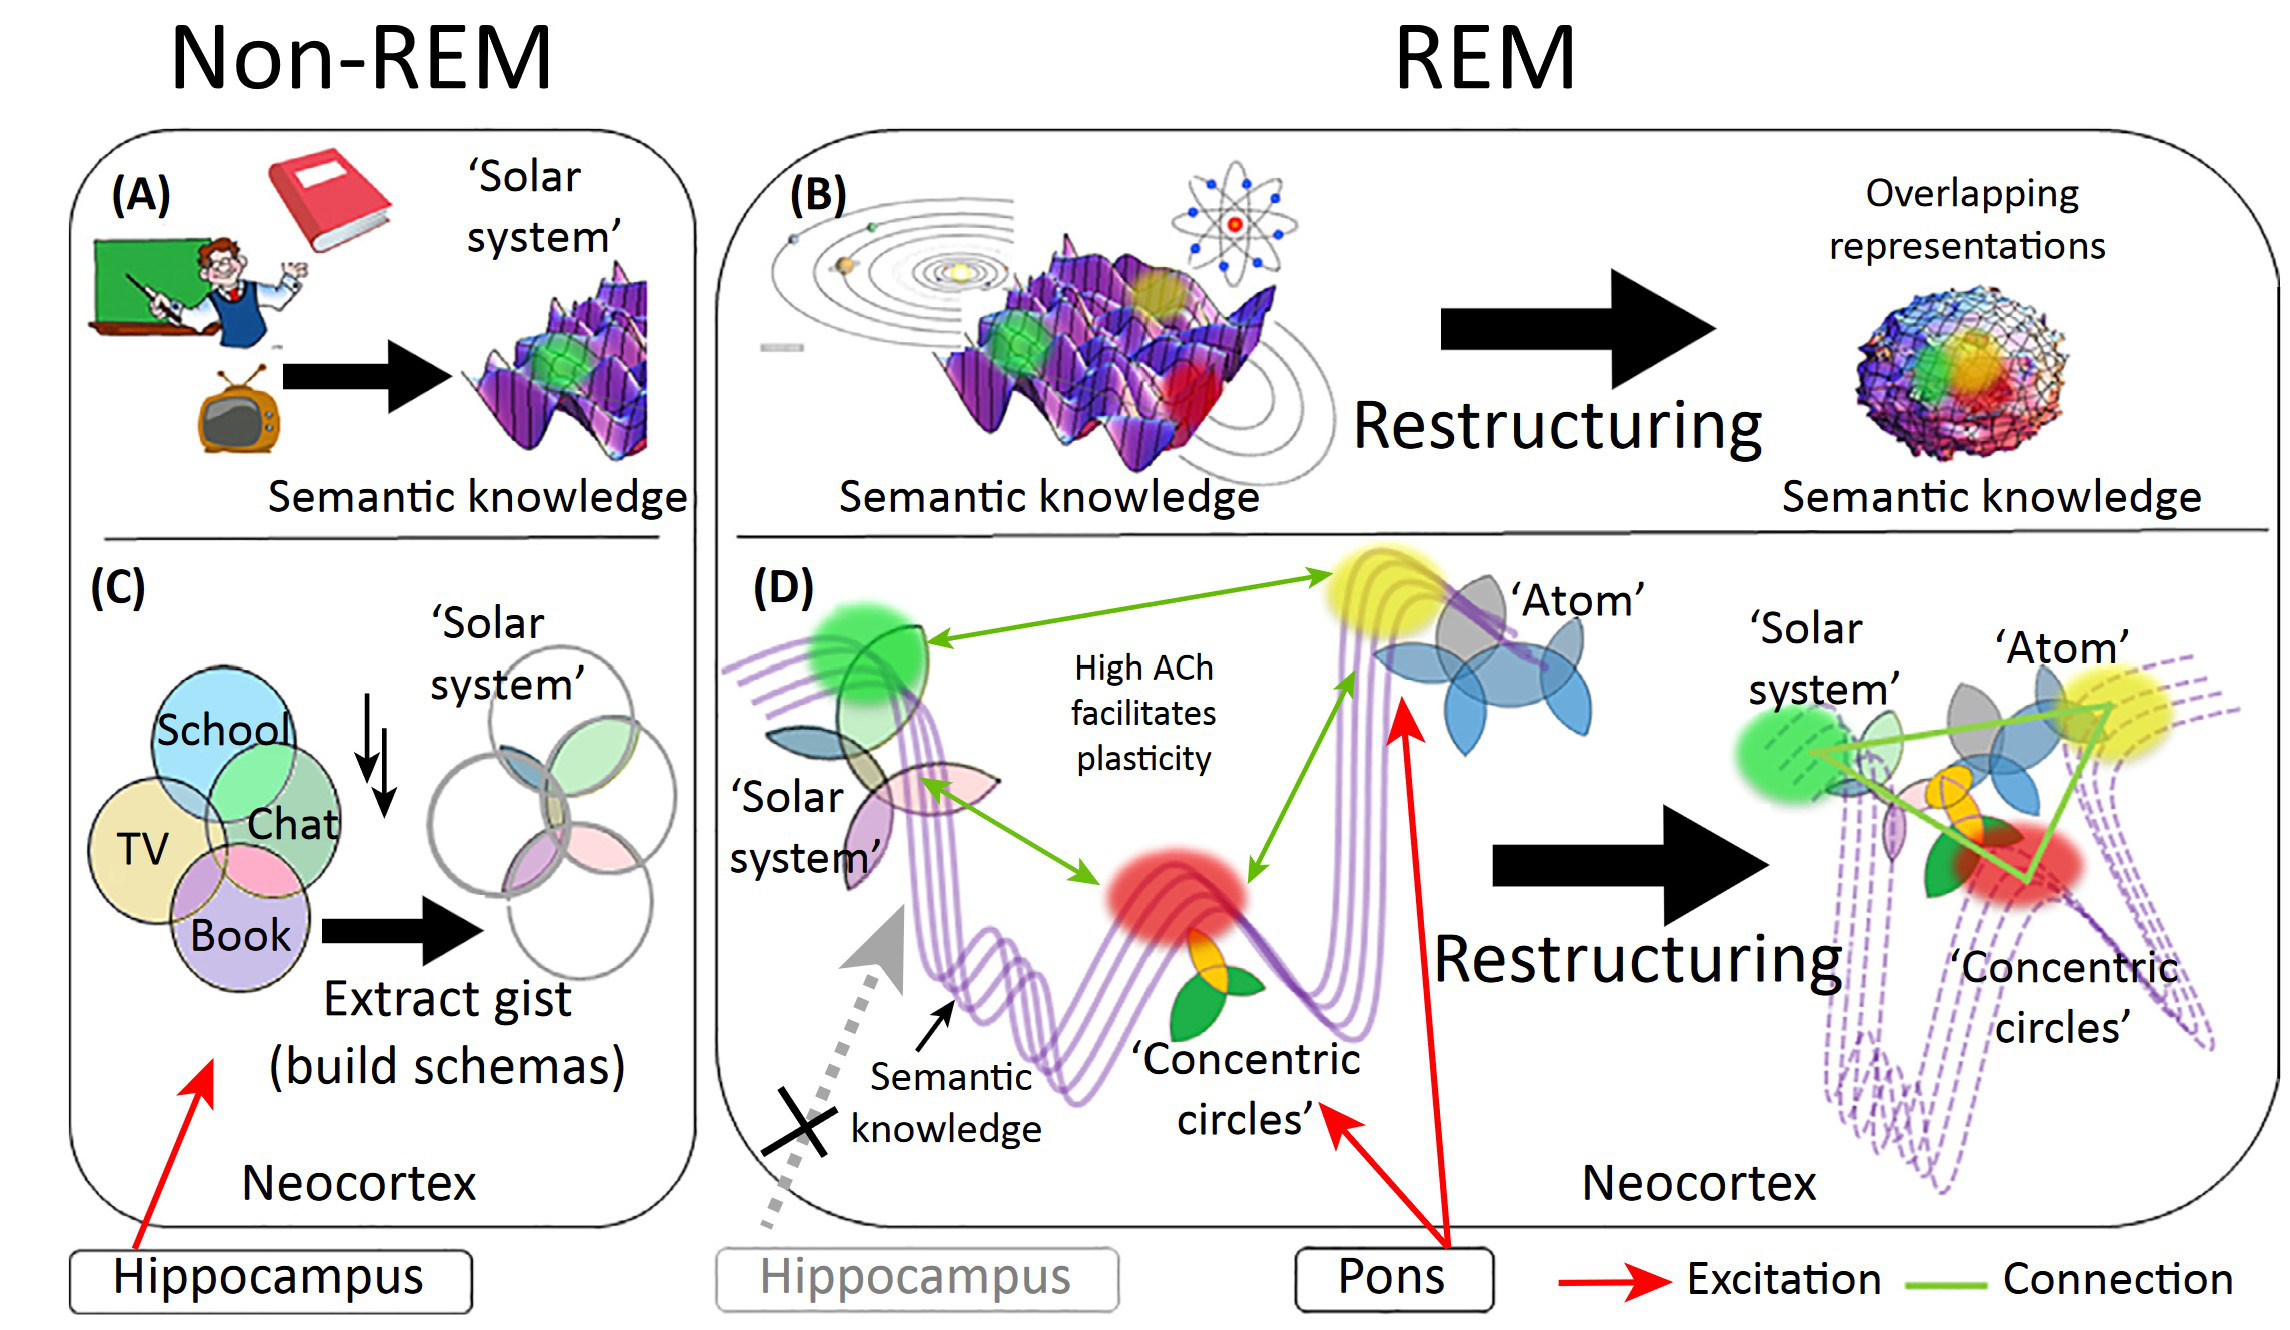
\includegraphics[width=0.9\linewidth]{1_Introduction//IntroImages/Picture6.jpg}
    \caption[\textit{The BiOtA model.}]{\textit{The BiOtA model.} \textbf{A} and \textbf{B} provide a simpler representation of \textbf{C} and \textbf{D}. \textbf{(A-C)} During NREM sleep, overlapping memories are replayed in the neocortex. Areas of overlap are strengthened, leading to general abstraction or the formation of new schemas. \textbf{(B-D)} During REM sleep, connections between the hippocampus and the neocortex are lost, and PGO waves trigger activity in other schemas, allowing the detection of similarities between schemas that, once found, lead to the restructure of knowledge. Modified from \cite{lewis_how_2018}.\vspace{1cm}}
    \label{fig:biota}
\end{figure}
\FloatBarrier

Finally, as briefly mentioned in Section \ref{Intro:sec:Memory processes}, a substantial body of research suggests that emotional memories are preferentially consolidated across sleep \parencite{alger_preferential_2018,cairney_targeted_2014,cunningham_psychophysiological_2014,groch_role_2013,hu_sleep_2006,nishida_rem_2009,tempesta_emotional_2015,wagner_brief_2006,wagner_emotional_2001}; however, see \parencite{lipinska_preferential_2019} that challenges this view. According to the \textbf{Sleep to Forget, Sleep to Remember Hypothesis} (SFSR), while the content (the information) of emotional memories is strengthened over time, the affective responses associated with their recall are attenuated across multiple nights of sleep \parencite{helm_overnight_2010,walker_role_2009}. It is therefore possible that time plays a vital role in modulating sleep’s impact on the visceral charge (emotional strength) of emotional memories. Moreover, the SFSR hypothesis also suggests that REM sleep, because of its unique biology, represents a particular brain state for the consolidation and modulation of emotional memories, and a variety of studies have confirmed this hypothesis \parencite{groch_role_2013,groch_dissociating_2015,harrington_influence_2018,helm_overnight_2010,hutchison_targeted_2021,nishida_rem_2009,menz_role_2013,menz_rem_2016,payne_sleep_2012,wagner_emotional_2001,wagner_brief_2006,wassing_restless_2019}.
Indeed, during REM sleep we observe (1) increased activity in limbic and paralimbic structures, which are key brain regions involved in the formation and consolidation of emotional memories; (2) theta oscillations, which propagation in limbic and prefrontal regions are believed to modulate affective experiences in both animals and humans; (3) increased concentrations of acetylcholine (ACh) - crucial for the long-term consolidation of emotional learning - and reduced concentration of noradrenergic and serotonergic input to the cortex, associated with lower levels of stress and anxiety \parencite[see] [for reviews]{walker_role_2009, helm_overnight_2010}.
\FloatBarrier
